
\section{Datenformat}\todo{Muss entweder noch umgeschrieben werden, wodurch es sehr lang wird oder massiv gekürzt werden. Ich warte noch auf Antwort von meinem Betreuer, Korrekturleser können bei 3.4 Datendarstellung weitermachen}
Die Daten liegen in einer Kombination aus sogenannten Python Dictionaries und sogennanten Python Listen vor.

Ein Dictionary ist dadurch charakterisiert, dass man über den Namen eines Elements (\glqq{}Key\grqq{}) das Element (\glqq{}Value\grqq{}) bekommt, ähnlich wie man früher in Telefonbüchern anhand des Namens (Key) die Telefonnummer (Value) erhalten hat.

Listen sind dadurch charakterisiert, dass sie Elemente in einer fixen Reihenfolge enthalten und sich diese durch ihren Index leicht auffindbar machen. So sind beispielsweise die Anzahl der COVID-19 Fälle der einzelnen Tage chronologisch in einer Liste gespeichert, sodass man daraus direkt eine Abbildung erstellen kann.


Die Programmdateien erstellen drei verschiedene sogenannte globale Dictionaries, welche (in untergeordneten Dictionaries und Listen) alle Daten enthalten. Globale Dictionaries sind in allen Dateien verfügbar und unterscheiden sich insofern von lokalen Dictionaries/Listen, welche nur in einzelnen Programmabschnitten vorliegen und daher nicht derart zentral sind.
Die drei Dictionaries heißen
\begin{itemize}
    \item covid19
    \item counties\_geography
    \item non\_county\_specific\_data
    \item districts
\end{itemize}

\textbf{covid19}\\
Das Dictionary covid19 speichert die COVID-19 Fälle jedes deutschen Landkreises und die daraus berechnete sieben Tages Inzidenz sowie die um den Mittelwert der 7-Tages Inzidenzen verminderten Inzidenzen.

Mit dem Gemeindeschlüssel eines Landkreises als Key und dem zusätzlichen Key \glqq{}cases\grqq{} erhält man die akkumulierte Anzahl an COVID-19 Fällen pro Tag des Landkreises als Liste.

Mit dem Gemeindeschlüssel eines Landkreises als Key und dem Key \glqq{}incidences\grqq{} erhält man die sieben Tages Inzidenz pro Tag des Landkreises als Liste.

Mit dem Gemeindeschlüssel eines Landkreises als Key und dem Key \glqq{}incidences\_scaled\grqq{} erhält man die sieben Tages Inzidenz pro Tag des Landkreises als Liste.

Alle drei Listen enthalten für jeden Tag seit dem 01.03.2020 bis zu dem Tag der aktuellsten Daten jeweils einen Eintrag.

Die Anzahl an COVID-19 Fällen pro Tag stammt aus dem \glqq{}COVID-19 Datenhub\grqq{}. Die sieben Tages Inzidenz wird wie in \autoref{sec:Grundlagen:7-Tages Inzidenz} beschrieben aus den Daten vom COVID-19 Datenhub berechnet.

\todo{Aufbau des Gemeindeschlüssels erklären}
\textbf{counties\_geography}\\
Das Dictionary counties\_geography enthält zu jedem Landkreis ein Dictionary mit den folgenden Elemente:
\begin{itemize}
    \item[name:] Der Name des Landkreises
    \item[population:] Die Einwohnerzahl des Landkreis aus einer offiziellen Schätzung (nähere Informationen finden sich im COVID-19 Datenhub). Diese Zahlen werden auch für die offizielle Berechnung der sieben Tages Inzidenz verwendet.
    \item[area\_in\_m2:] Die Fläche des Landkreises in Quadratmetern
    \item[geometry:] Die Form des Landkreises in einer für die Darstellung angepassten Form
    \item[raw\_geometry:] Die Form des Landkreises in der originalen Form
    \item[population\_density:] Die Bevölkerungsdichte des Landkreises, berechnet aus der Fläche des Landkreises und seiner Einwohnerzahl
\end{itemize}
Außer die Bevölkerungsdichte, welche berechnet wird, und die angepassten Formen der Landkreise, welche aus den origialen Formen generiert werden, stammen alle Daten direkt aus dem \glqq{}COVID-19 Datenhub\grqq{}.

\textbf{non\_county\_specific\_data}
Das Dictionary non\_county\_specific\_data enthält die folgenden Elemente:
\begin{itemize}
    \item[unixtime:] Die Unixzeit, wie sie vom COVID-19 Datenhub zur Verfügung gestellt wird: Die Zahl der Millisekunden seit dem 01.01.1970 00:00 Uhr UTC. Die Zahl der COVID-19 Fälle und die sieben Tages Inzidenz eines entsprechenden Tages befinden sich an der selben Stelle in Ihrer jeweiligen Liste, wie der Tag in dieser Liste.
    \item[states:] Die Name und Nummern der deutschen Bundesländer. Die ersten beiden oder die erste Zahl des Gemeindeschlüssel eines Landkreises geben das Bundesland an, in welchem der Landkreis liegt. Die ersten zwei bzw. drei Zahlen geben den Regierungsbezirk an, in dem der Landkreis. Sollte es im jeweiligen Bundesland keine Regierungsbezirke geben, entspricht dies dem Bundesland.
    \item[highest\_case\_number:] Die höchste akkumulierte Fallzahl unter allen Landkreisen.
    \item[lowest\_case\_number:] Die niedrigste akkumulierte Fallzahl unter allen Landkreisen.
    \item[highest\_incidence:] Die höchste sieben Tages Inzidenz eines Tages unter allen Landkreisen.
    \item[lowest\_incidence:] Die niedrigste sieben Tages Inzidenz eines Tages unter allen Landkreisen.
    \item[UTC:] Die Unixzeit konvertiert in die Koordinierte Weltzeit im Format \glqq{}DD.MM.YYYY\grqq{}.
    \item[UTC+7days:] Die Liste der Zeiten gespeichert in UTC plus sieben weitere Tage vor dem erstem Datum in der Liste. Diese werden benutzt, um den Zeitraum der 7-Tages Inzidenz der ersten sieben Tage darstellen zu können: die hierfür verwendeten Zeiträume beginnen jeweils vor dem ersten hier dokumentierten Fall.
\end{itemize}
\todo{itemize reparieren}
Die Unixzeit, die Namen und die Nummern der Bundesländer stammen aus dem \glqq{}COVID-19 Datenhub\grqq{}. Alle anderen Informationen wurden gesammelt oder berechnet.

In Abbildung \ref{fig:dicts_als_code} sind die drei Dictionaries dargestellt, wie sie auch im Programm verwendet werden.
\begin{figure}[H]
    \centering
    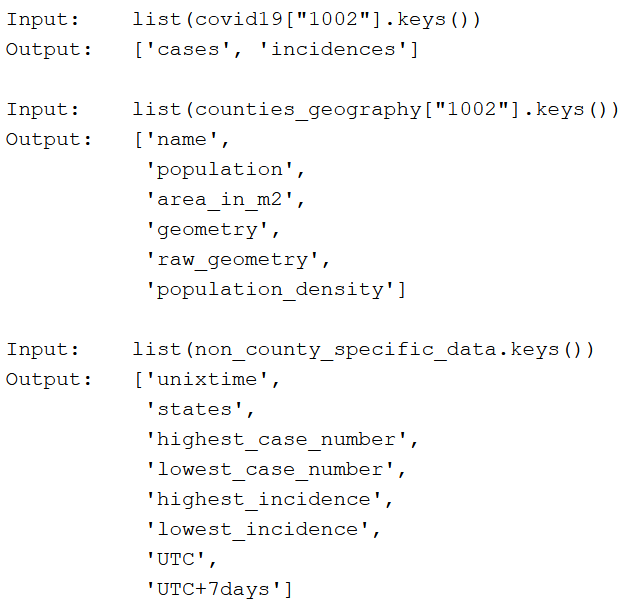
\includegraphics[width=0.8\textwidth]{figures/Vorgehensweise/Dictionarys Bachelorprojekt.png}
    \caption{
    Die Dictionaries non\_county\_specific\_data, counties\_geography und covid19 mit ihren jeweiligen Schlüsseln.
    Für die Dictionaries covid19 und counties\_geography wurde jeweils der Landkreis Kiel (Gemeindeschlüssel 1002) zur Veranschaulichung verwendet.}
    \label{fig:dicts_als_code}
\end{figure}

\todo{Daten aus Meldungen einpflegen}